\subsection{Multi-Model Component}
\label{sec:architecture_multicomponent}

The \texttt{MultiComponent} abstraction extends the component interface to several interchangeable model realizations of one physical subsystem.
It exposes one public component interface to the surrounding \texttt{System} and delegates execution to one active internal model.
This supports runtime switching between models with different fidelity levels or modeling approaches.

Figure~\ref{fig:multi_component} shows the public interface, the internal model registry, and the switching-support responsibilities.

\begin{figure}[t]
  \centering
  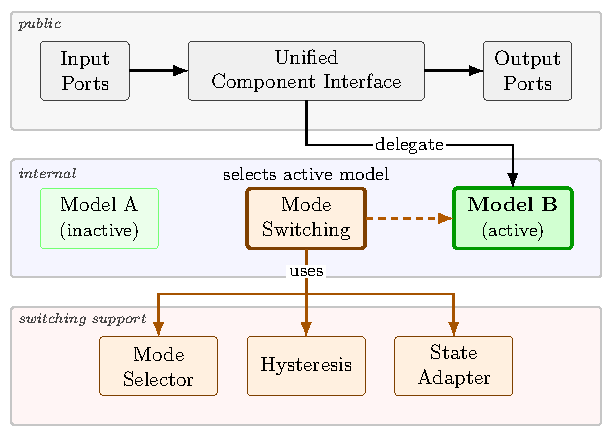
\includegraphics[width=0.7\textwidth]{figures/4_architecture/multi_model.pdf}
  \caption[Architectural view of the \texttt{MultiComponent} abstraction]{Architectural view of the \texttt{MultiComponent} abstraction.
  The wrapper exposes one unified component interface and delegates execution to one active model from a registered set.
  A mode selector, hysteresis, and state adapter together change the active model when the switching criteria require it.}
  \label{fig:multi_component}
\end{figure}

At any point in time, exactly one internal model is active.
The active model provides the outputs exposed by the wrapper and receives the delegated lifecycle and stepping calls.
Inactive models remain registered inside the wrapper so that they can become active later without changing the surrounding system structure.

A switch changes the active model.
The mode selector determines the requested model from the switching criteria defined by the concrete component.
Hysteresis enforces a minimum dwell time between consecutive switches and suppresses rapid changes near switching boundaries.
The state adapter maps the physical state exported by the outgoing model to a representation accepted by the incoming model.

The abstraction separates model choice from system assembly.
The surrounding \texttt{System} connects only to the public interface of the \texttt{MultiComponent}.
The implementation details of port unification, state transfer, and switching are described in Section~\ref{sec:impl_multi_model}.